\section{Data selection}
\lb{sec:data}


\begin{figure*}[h]
%\centering
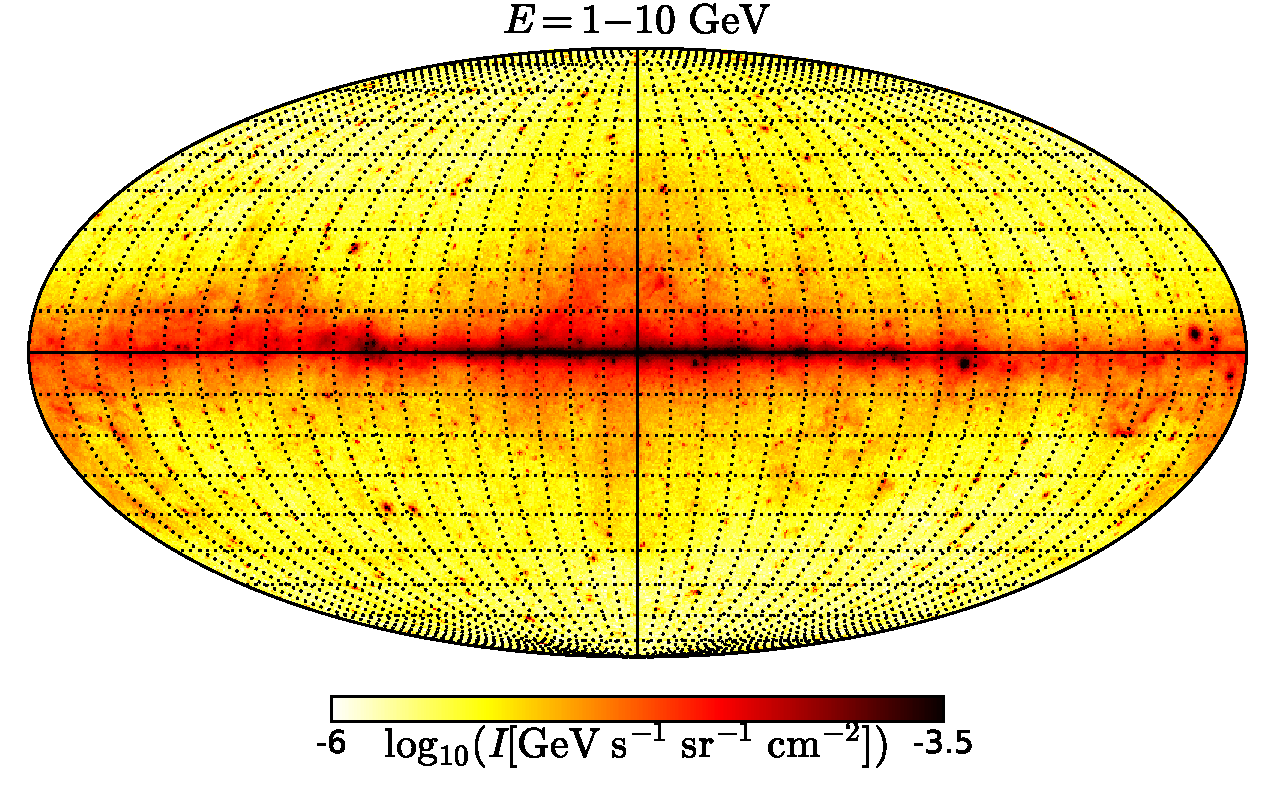
\includegraphics[width=0.33\textwidth]{plots/Mollweide_data_source_range_0.pdf}
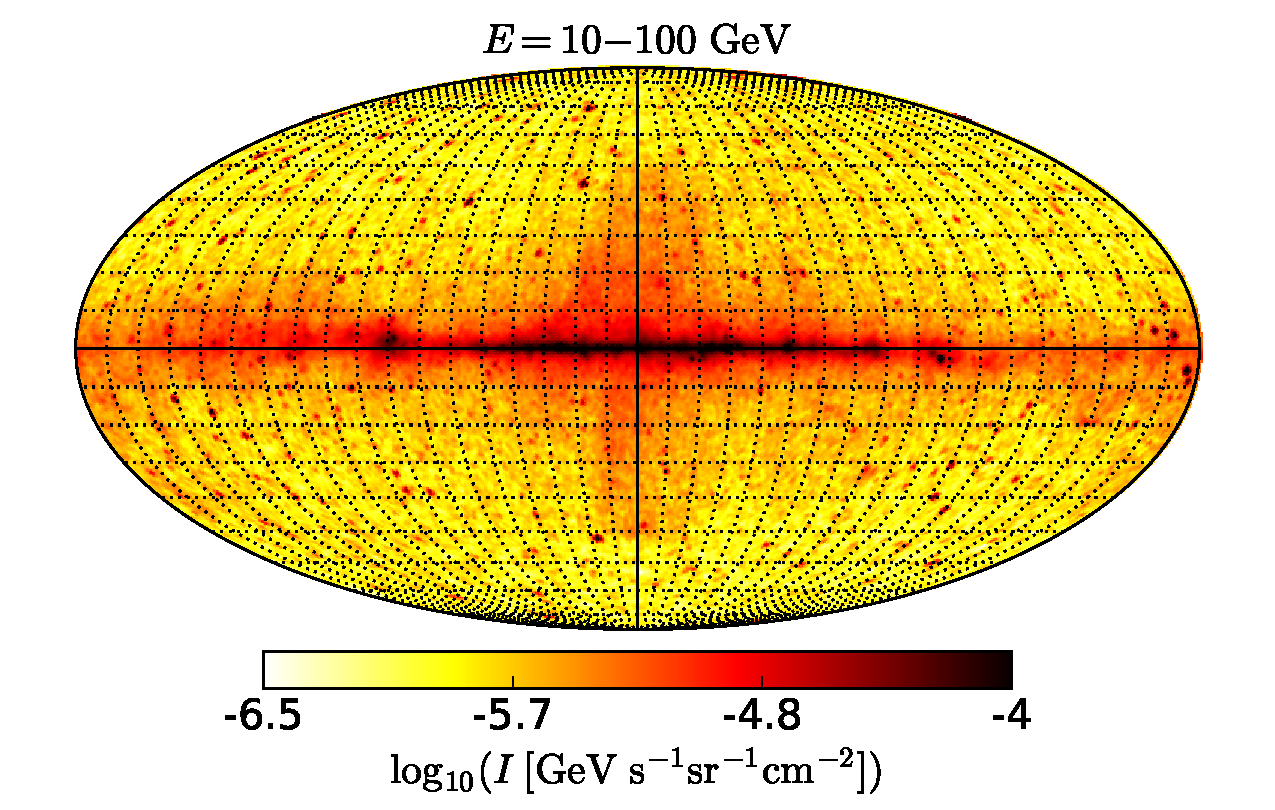
\includegraphics[width=0.33\textwidth]{plots/Mollweide_data_source_range_1.pdf}
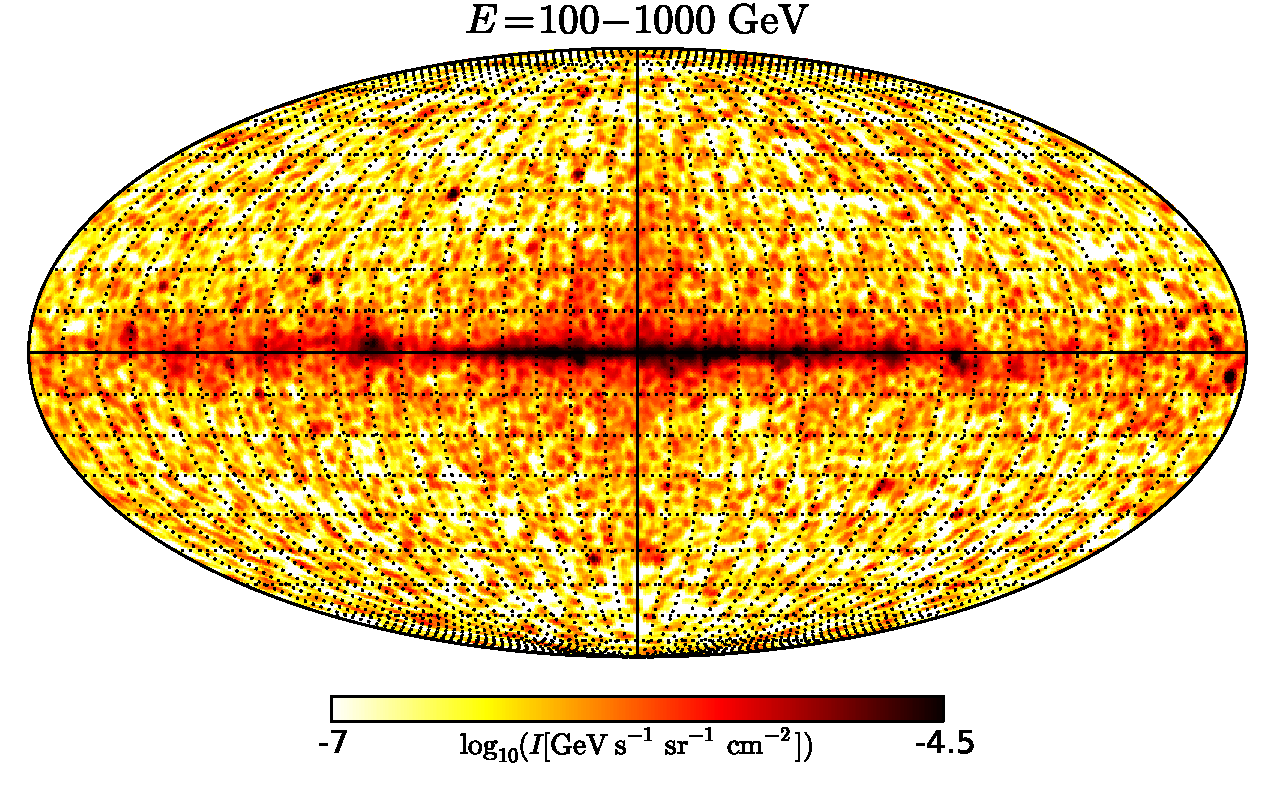
\includegraphics[width=0.33\textwidth]{plots/Mollweide_data_source_range_2.pdf}
\caption{
Energy flux of the \Fermi-LAT 9 years of Source class data integrated in energy ranges 1 -- 10 GeV, 10 -- 100 GeV, and 100 GeV -- 1 TeV.
The maps are represented in logarithmic scale. 
The map in the energy range 10 -- 100 GeV (100 -- 1000 GeV) 
is smoothed with a Gaussian kernel with radius $\sigma = 0^\circ\!\!.5$ ($\sigma = 0^\circ\!\!.7$).
The plots are created with the \Healpix package \citep{2005ApJ...622..759G}, Mollweide projection, 
nside = 128 ($\approx 0\degr\!\!.46$ pixel size). 
}
\label{fig:Maps_data}
\end{figure*}

%The main goal of the analysis is a study of a relatively small region $\lesssim 10^\circ$ from the GC for energies $\gtrsim 1$ GeV.
We use 9 years of the \Fermi-LAT Pass 8 Source class events
between August 4, 2008  and August 3, 2017 ({\Fermi} Mission Elapsed Time 239557418\,s -- 523411376\,s)
with energies between 316 MeV $ = 10^{2.5}$ MeV
and 1 TeV separated in 21 logarithmic energy bins (6 bins per decade).
The selection of the events is performed with the standard quality cuts (DATA\_QUAL$>$0)\&\&(LAT\_CONFIG==1).
In order to avoid contamination from gamma rays produced in interactions of CR in the Earth atmosphere, 
we select events with zenith angles $\theta < 100^{\circ}$,
which is sufficient for energies above 316 MeV.
We calculate the exposure and point-spread function (PSF) using the {\Fermi}-LAT Science Tools package version 
10-01-01 available from the {\Fermi} Science Support Center\footnote{\url{http://fermi.gsfc.nasa.gov/ssc/data/analysis/}} 
with the P8R2\_SOURCE\_V6 instrument response functions.
Figure \ref{fig:Maps_data} shows the energy flux of the gamma-ray emission
integrated in three energy ranges%
\footnote{The integral of the energy flux intensity between $E_0$ and $E_1$ is defined as
$I = \int_{E_0}^{E_1} E \frac{dN}{dE} dE.$}.
For all maps shown in this paper, we use Galactic coordinates centered on the GC in Mollweide projection. %The graticule spacing is $\ang{10}$ in latitude and longitude. 
%The maps are smoothed with a $\sigma = \ang{0.5}$ Gaussian kernel.
For spatial binning we use \Healpix\footnote{\url{http://sourceforge.net/projects/healpix/}} \citep{2005ApJ...622..759G} scheme with a pixelization of order 7  
($\approx 0\degr\!\!.46$ pixel size). 

